%
\documentclass{article} % For LaTeX2e
\usepackage{nips13submit_e,times}
\usepackage{hyperref}
\usepackage{algorithmicx}
\usepackage[ruled,vlined]{algorithm2e}
\usepackage{url, tikz}
\usepackage[justification=centering]{subcaption}
\usepackage[margin=1in]{geometry}
\usepackage{amsmath,amssymb}
\usepackage{mathtools}
\usepackage{pgfplots}
\usepackage{booktabs}
\usetikzlibrary{bayesnet}
\pgfplotsset{compat=newest}

%\documentstyle[nips13submit_09,times,art10]{article} % For LaTeX 2.09

\newcommand\fixme[1]{\textcolor{red}{#1}}

\newenvironment{loglisting}[1][htb]
{\renewcommand{\algorithmcfname}{Log listing}% Update algorithm name
  \begin{algorithm}[#1]%
}{\end{algorithm}}

\makeatletter
\algrenewcommand\ALG@beginalgorithmic{\ttfamily}
\makeatother

\title{
Click models evaluations\\
\small {(IR2 project)}
}

\author{
Luka Stout\\
\texttt{10616713} \\
\and
Finde Xumara \\
\texttt{10690832} \\
}

\newcommand{\fix}{\marginpar{FIX}}
\newcommand{\new}{\marginpar{NEW}}
\newcommand{\comment}[1]{\textit{\color{red}{#1}}}

\nipsfinalcopy % Uncomment for camera-ready version

\begin{document}

\nocite{*}
\maketitle

%\begin{abstract}
%\end{abstract}

\section{Introduction}
Modeling user behavior on a search engine result page is important for understanding users and supporting simulation experiments.
As result pages become more complex, click models have to evolve as well in order to capture additional aspects of user behavior in response to new forms of result presentation.
In recent years many models have been proposed that are aimed at predicting behaviour of web search users. 

In this project, we implement and evaluate different click models using multiple evaluation metrics and report on the performance of these click models.
The click models include the Click-Through Rate click model (CTR), Position-Based click model (PBM), Cascade click model (CM) \cite{Kempe2008}, \fixme{Dependent Click Model (DCM) \cite{Guo2009_DCM}, Dynamic Bayesian Network click model (DBN) \cite{Chapelle2009}}, User Browsing Model (UBM) \cite{Dupret2008}, Click Chain Model (CCM) \cite{Guo2009_CCM} and Task-centric Click Model (TCM) \cite{Zhang2011}.
The evaluation metrics we use to evaluate performance of these click models are loglikelihood, perplexity, click-through-rate prediction, relevance prediction, ranking performance and computation time. We will also analyze two different factors that might influence performance of the click models, query frequency and click entropy.
By doing this experiment we will know the performance of each different click model and this information can be helpful in the creation of new click models and used as a performance benchmark of new click model proposals.

%report organization
This report is organized as follows.
In Section~\ref{sec:methodology} we will describe different click models and evaluation algorithms used in our experiments.
The experiments and data source information will be covered in Section~\ref{sec:evaluation}, followed by an analysis of these experiments in Section~\ref{sec:analysis}.

\section{Methodology}
\label{sec:methodology}
We compare UBM, DCM, DBN and TCM on the Yandex dataset \cite{yandex}. In this section, we briefly describe their main characteristics and differences. We have implemented TCM ourselves, the other algorithms were taken from PyClick \cite{PyClick}.

\subsection{DCM}
The dependent click model was first proposed by Guo et al. in \cite{Guo2009}. In the paper they propose a new click model which can handle multiple clicks per query by introducing a position dependent parameter $lambda_j$ to reflect the chance that the user would like to see more results after a click at position $j$. A graphical representation of the model is presented in Figure\ref{fig:dcm_gm} 

\subsection{DBN}
The dynamic bayesian network is an extension to the traditional cascade model proposed by Chapelle and Zhang in \cite{Zhang2011}. For a given position $j$, in addition to observed variable $C_j$ indicating whether there was a click or not at this position, the following latent variable are defined to model examination, perceived relevance and actual relevance, respectedly:
\begin{itemize}
	\item $E_j$: did the user $examine$ the document?
	\item $A_j$: was the user $attracted$ by the document?
	\item $S_j$: was the user $satisfied$ by the clicked document?
\end{itemize}
They introduce a variable $s_u$ for each document $u$ which describes the relevance of the document for this query. When the user clicks on this document, there is a certain chance that the user will be satisfied. If the user is not satisfied, he continues to examine the next document with a probability $\gamma$ and stops otherwise. The parameter $\gamma$ is known as the 'perseverance'. A graphical representation of the model is presented in Figure \ref{fig:dbn_gm}. 

\begin{figure}[ht!]
	\begin{subfigure}[b]{.45\textwidth}
		\centering
		\input{graph/model_dcm}
		\caption{DCM}	
		\label{fig:dcm_gm}
	\end{subfigure}
	\begin{subfigure}[b]{.45\textwidth}
		\centering
		\input{graph/model_dbn}
		\caption{DBN}
		\label{fig:dbn_gm}
	\end{subfigure}
	\caption{The graphical model of DCM and DBN.}
\end{figure}

\subsection{UBM}
In \cite{Dupret2008}, Dupret and Piwowarski propose a new click model called the User Browsing Model (UBM). The main difference between UBM and other models is that UBM takes the distance into account from the current document \(u_j\) to the last clicked document \(u_{j'}\) for determining the probability that the user continues browsing:
\[P(E_j =1 \mid C_{j'}=1, C_{j'+1}=0, \dots, C_{j-1}=0) = \gamma_{jj'}\]
The probability that a document at rank \(j\) is examined \(E_j\) therefore depends on all possible paths the user could have taken to arrive at this document:
\[P(E_j = 1) = \sum_{j'=1}^{j-1} \gamma_{jj'}\]
A graphical representation of the model is presented in Figure~\ref{fig:ubm_gm}.

\begin{figure}[ht!]
	\begin{center}
		\begin{tabular}{c}
			\input{graph/model_ubm}
		\end{tabular}
	\end{center}
	\caption{The graphical model of UBM.}	
	\label{fig:ubm_gm}
\end{figure}

\subsection{TCM}
The Task-centric Click Model (TCM) was first proposed by Zhang et al. in \cite{Zhang2011}. In the paper they propose a new click model which can handle multiple clicks of multiple queries in a task by introducing two new biases. The first bias indicates that users tend to express their information needs incrementally in a task, thus perform more clicks as their needs become clearer. The other bias indicates that users tend to click fresh documents that are not included in the results of previous queries. In their paper, they named the first assumption as \texttt{query bias}, and the second assumption as \texttt{duplicate bias}. A graphical representation of the state-of-the-art of the model is presented in Figure\ref{fig:dcm_gm} and the notations used in TCM are described in Table\ref{table:tcm_notations}. 

\begin{table}[ht]
	\centering
	\begin{tabular}{l|lll|}
		\hline
		Symbol & Description \\
		\hline
		(\(i\),\(j\)) 	& \(j\)-th ranking position in \(i\)-th query session.\\
		$M_i$			& Whether the \(i\)-th query matches the user's intent.\\
		$N_i$ 			& Whether the the user submits another query after \(i\)-th query session.\\		
		$E_{i,j}$ 		& Examination of the document at (\(i\),\(j\)).\\
		$H_{i,j}$ 		& Previous Examination of the document at (\(i\),\(j\)).\\
		$F_{i,j}$ 		& Freshness of the document at (\(i\),\(j\)).\\
		$R_{i,j}$ 		& Relevance of the document at (\(i\),\(j\)).\\
		$C_{i,j}$ 		& Whether the the document at (\(i\),\(j\)) is clicked.\\
		(\(i'\),\(j'\)) & Assume that \(d\) is the document at (\(i\),\(j\)).\\
		&\(i'\) is the latest query session where \(d\) has appeared in previous query sessions,\\ &and \(j'\) is the ranking position of this appearance.\\
		\hline
	\end{tabular}
	\caption{Notations used in TCM}
	\label{table:tcm_notations}
\end{table}

\begin{figure}[ht!]
	\begin{center}
		\begin{tabular}{c}
			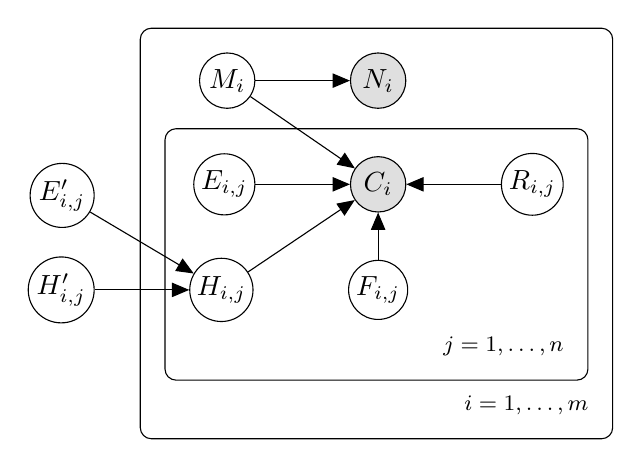
\begin{tikzpicture}

  % Define nodes
  \node[obs]                      (n) {$N_i$};
  \node[latent, left=1.2cm of n]  (m) {$M_i$};
  \node[obs, below=0.6cm of n]    (c) {$C_i$};
  \node[latent, left=1.2cm of c]  (e) {$E_{i,j}$};
  \node[latent, right=1.2cm of c] (r) {$R_{i,j}$};
  \node[latent, below=0.6cm of c] (f) {$F_{i,j}$};
  \node[latent, left=1.2cm of f]  (h) {$H_{i,j}$};
  \node[latent, left=1.2cm of h]  (h_prime) {$H_{i,j}'$};
  \node[latent, left=1.2cm of h, yshift=1.2cm]  (e_prime) {$E_{i,j}'$};

  % Connect the nodes
  \edge {m} {n,c} ; %
  \edge {e,r,f} {c} ; %
  \edge {h} {c} ; %
  \edge {h_prime,e_prime} {h} ; %

  % Plates
  \plate [inner sep=.3cm] {p_n} {(e)(c)(r)(f)(h)} {$j=1,\dots,n$} ;
  \plate [inner sep=.3cm] {p_m} {(m)(n)(p_n)} {$i=1,\dots,m$} ;

\end{tikzpicture}
		\end{tabular}
	\end{center}
	\caption{The graphical model of state-of-the-art TCM.}
	\label{fig:tcm_gm}
\end{figure}

This model can be formalized with the following conditional probabilities:
\begin{align}
	P(M_i=1) &= \alpha_1 \\
	\label{eq:alpha_2}
	P(N_i|M_i=1) &= \alpha_2 \\
	P(F_{i,j}=1|M_{i,j}=1) &= \alpha_3 \\
	P(E_{i,j}=1) &= \beta_j \\
	P(R_{i,j}=1) &= r_d \\
	M_i = 0 &\Rightarrow N_i = 1\\
	H_{i,j} = 0 &\Rightarrow F_{i,j} = 1\\
	H_{i,j} = 0 &\Leftrightarrow H_{i',j'} = 0, E_{i',j'} = 0\\
	C_{i,j} = 1 &\Leftrightarrow M_i = 1, E_{i,j} = 1, R_{i,j} = 1, F_{i,j} = 1
\end{align}


In our implementation, we simplified TCM model by assuming that $M_i$ is observed from the click log data, thus eq.\ref{eq:alpha_2} can be removed.
Our second assumptions is that $M_i, E_{i,j},R_{i,j}$ and $F_{i,j}$ are independent.
The graphical model of our TCM implementation is presented in Fig \ref{fig:tcm_gm_new}.
\begin{figure}[ht!]
	\begin{center}
		\begin{tabular}{c}
			\input{graph/model_tcm_new}
		\end{tabular}
	\end{center}
	\caption{The graphical model of simplified TCM.}
	\label{fig:tcm_gm_new}
\end{figure}

The simplified TCM can be formularized with the following conditional probabilities.

\subsubsection{Click probability}
For $P(F_{i,j}=1)$ we introduce a variable $f_{i,j}$, which will be derived later. \\
By assumption that $M_i, E_{i,j},R_{i,j}$and$F_{i,j}$ are independent, click probability can be formularize as:
\begin{align}
	P(C_{i,j} = 1)
	&= P(M_i=1) * P(E_{i,j}=1) * P(R_{i,j}=1) * P(F_{i,j} = 1) \\
	&= \alpha_1 * \beta_j * r_{i,j} * f_{i,j}
	\label{eq:proba_click}
\end{align}

\subsubsection{Probability of the query match user intention}
Because we remove equation that depends on $\alpha_2$, we can now set $\alpha_1$ as MLE.
\begin{align*}
	P(M_i = 1) 
	&= \alpha_1 \\
\end{align*}

\subsubsection{Probability of user submit next query}
User submit next query if the query does not match user intention ($\alpha_1$) or user want to search more.
\begin{align*}
	P(N_i=1) 
	&= \frac{1}{|S|} \sum_{i\in S} \mathcal{I}(N_i=1) \\
	&= \frac{q_i}{|S|} \\
	&= n_i
\end{align*}

$q_i$ is the number of submitted-queries where user submit another query after $i$-th query session.

\begin{align*}
	P(N_i=1|M_i=1) 
	&= \alpha_2 \\
	&= \frac{P(N_i=1) - P(N_i=1|M_i=0)P(M_i=0)}{P(M_i=1)} \\
	&= \frac{n_i + \alpha_1 - 1}{\alpha_1}
\end{align*}

\subsubsection{Relevance probability}
\begin{align*}
	P(R_{i,j} = 1)
	&= r_{i,j} \\
	&= \frac{\sum_{q_{i,j} \in S_{i,j}} P(R_{i,j}=1 | C)}{|S_{i,j}|}
\end{align*}

Where $S_{i,j}$ are all sessions (queries) containing the document corresponding with the query $i$ at rank $j$ - document
$P(R_{i,j}=1 | C)$ will be derive on eq.\ref{eq:proba_relevant_given_click}

\begin{align}
	P(R_{i,j}=1 | C)
	&= \mathcal{I}(C_{i,j} = 1) P(R_{i,j}|C_{i,j}=1) + \mathcal{I}(C_{i,j} = 0) P(R_{i,j}|C_{i,j}=0) \\
	&= c_{i,j} + (1-c_{i,j}) \frac {P(C_{i,j}=0|R_{i,j}=1) P(R_{i,j} = 1)} {P(C_{i,j} = 0)} \\
	&= c_{i,j} + (1-c_{i,j}) \frac {P(C_{i,j}=0|R_{i,j}=1) r_{i,j}} { 1 - P(C_{i,j} = 1)}
	\label{eq:proba_relevant_given_click}
\end{align}
Where $c_{i,j} = 1$ if (i,j) was clicked in the current session.
$P(C_{i,j}=0|R_{i,j}=1)$ is the chance of no click given that it is relevant. 

\begin{align*}
P(C_{i,j}=0|R_{i,j}=1) 
	&= P(C_{i,j }=0|R_{i,j}=1, M_i = 1) P(M_i=1) + P(C_{i,j }=0|R_{i,j}=1, M_i = 0)P(M_i=0) \\
	&= \alpha_1 P(C_{i,j }=0|R_{i,j}=1, M_i = 1, E_{i,j}=1) P(E_{i,j}=1)\\     &+ \alpha_1 P(C_{i,j }=0|R_{i,j}=1, M_i = 1, E_{i,j}=0) P(E_{i,j}=0)\\
	&+ (1-\alpha_1) P(C_{i,j }=0|R_{i,j}=1 , M_i = 0, E_{i,j}=1) P(E_{i,j}=1)\\
	&+ (1-\alpha_1) P(C_{i,j }=0|R_{i,j}=1 , M_i = 0, E_{i,j}=0) P(E_{i,j}=0) \\
	\\
	&= \alpha_1 \beta_j P(C_{i,j }=0|R_{i,j}=1, M_i = 1, E_{i,j}=1, F_{i,j}=1) P(F_{i,j}=1)\\
	&+ \alpha_1 \beta_j P(C_{i,j }=0|R_{i,j}=1, M_i = 1, E_{i,j}=1, F_{i,j}=0) P(F_{i,j}=0)\\
	&+ \alpha_1 (1-\beta_j) P(C_{i,j }=0|R_{i,j}=1 , M_i = 1, E_{i,j}=0, F_{i,j}=1) P(F_{i,j}=1)\\
	&+ \alpha_1 (1-\beta_j) P(C_{i,j }=0|R_{i,j}=1 , M_i = 1, E_{i,j}=0, F_{i,j}=0) P(F_{i,j}=0)\\
	&+ (1-\alpha_1) \beta_j P(C_{i,j }=0|R_{i,j}=1, M_i = 0, E_{i,j}=1, F_{i,j}=1) P(F_{i,j}=1)\\
	&+ (1-\alpha_1) \beta_j P(C_{i,j }=0|R_{i,j}=1, M_i = 0, E_{i,j}=1, F_{i,j}=0) P(F_{i,j}=0)\\
	&+ (1-\alpha_1) (1-\beta_j) P(C_{i,j }=0|R_{i,j}=1 , M_i = 0, E_{i,j}=0, F_{i,j}=1) P(F_{i,j}=1)\\
	&+ (1-\alpha_1) (1-\beta_j) P(C_{i,j }=0|R_{i,j}=1 , M_i = 0, E_{i,j}=0, F_{i,j}=0) P(F_{i,j}=0)\\
\end{align*}
We note that $P(C_{i,j }=0|R_{i,j}=1, M_i = 1, E_{i,j}=1, F_{i,j}=1) = 0$. Otherwise it is $1$. From eq. 24 from TCM paper. Together with inserting our parameters this gives us the following:

\begin{align}
	P(C_{i,j}=0|R_{i,j}=1) &= 
	\alpha_1 \beta_j f_{i,j} +
	\alpha_1 \beta_j (1-f_{i,j}) + 
	\alpha_1 (1-\beta_j) f_{i,j} +
	\alpha_1 (1-\beta_j) (1-f_{i,j}) \\
	&+ (1-\alpha_1) \beta_j f_{i,j} +
	(1-\alpha_1) \beta_j (1-f_{i,j}) +
	(1-\alpha_1) (1-\beta_j) (f_{i,j} \\
	&+(1-\alpha_1) (1-\beta_j) (1-f_{i,j})
\end{align}

expanding this we are only left with
\begin{align}
	P(C_{i,j}=0|R_{i,j}=1) = 1 - (\alpha_1 \beta_j f_{i,j})
	\label{eq:chance_no_click_given_relevant}
\end{align}
Which seems intuitive as we assumed that all $M_i, R_{i,j}, E_{i,j}$ and $F_{i,j}$ are independent to get $P(C_{i,j} = 1)$ . With this information we can calculate 
\begin{align}
	P(R_{i,j}=1 | C) &= c_{i,j} + (1-c_{i,j}) \frac { (1 - (\alpha_1 \beta_j f_{i,j}))  r_{i,j}} { 1 - \alpha_1 \beta_j f_{i,j} r_{i,j} } \\
	&= c_{i,j} + (1-c_{i,j}) \frac{r_{i,j} - \alpha_1 \beta_j f_{i,j} r_{i,j} }{ 1 - \alpha_1 \beta_j f_{i,j} r_{i,j}}
\end{align}

\subsubsection{Examination probability}
\begin{align}
	P(E_{i,j} = 1) 
	&= \beta_j \\
	&= \frac{1}{|S|} \sum_{i \in S} P(E_{i,j}=1 | C)
\end{align}
Where $S$ is all sessions and $i$ is a query within that session.
$P(E_{i,j}=1 | C)$ will be derive on eq.\ref{eq:proba_examined_given_click}

\begin{align}
	\label{eq:proba_examined_given_click}
	P(E_{i,j}=1 | C)
	&= \mathcal{I}(C_{i,j} = 1) P(E_{i,j}|C_{i,j}=1) + \mathcal{I}(C_{i,j} = 0) P(E_{i,j}|C_{i,j}=0) \\
	&= c_{i,j} + (1-c_{i,j}) \frac {P(C_{i,j}=0|E_{i,j}=1) P(E_{i,j} = 1)} {P(C_{i,j} = 0)} \\
	&= c_{i,j} + (1-c_{i,j}) \frac {P(C_{i,j}=0|E_{i,j}=1) \beta_j} { 1 - P(C_{i,j} = 1)}
\end{align}
Where $c_{i,j}$ indicates whether document $i,j$ was clicked.
Analog to eq \ref{eq:chance_no_click_given_relevant} we can show that
\begin{align}
	P(C_{i,j}=0|E_{i,j}=1) = 1 - (\alpha_1 f_{i,j} r_{i,j})
\end{align}

This gives us 
\begin{align}
	P(E_{i,j}=1 | C) 
	&= c_{i,j} + (1-c_{i,j}) \frac {( 1 - (\alpha_1 f_{i,j} r_{i,j}) )\beta_j} { 1 - \alpha_1 \beta_j f_{i,j} r_{i,j}} \\
	& = c_{i,j} + (1-c_{i,j}) \frac {\beta_j - \alpha_1 \beta_j f_{i,j} r_{i,j}} { 1 - \alpha_1 \beta_j f_{i,j} r_{i,j}}
\end{align}

\subsubsection{Freshness probability}
\begin{align}
	P(F_{i,j} = 1 | H_{i,j} = 1) &= \alpha_3 \\
	\alpha_3 &= \frac{1}{|S_{i,j}|} \sum_{q \in S} \sum_{(i,j) \in q} P(F{i,j}=1 | H_{i,j}=1, C)
	\label{eq:freshness}
\end{align}

Where (i,j) is a query, rank pair identifying a certain document.
$P(F_{i,j}=1 | C)$ will be derive on eq.\ref{eq:proba_freshness_given_click} \\
$P(F_{i,j}=1)$ will be derive on eq.\ref{eq:proba_freshness}

\begin{align}
	\label{eq:proba_freshness_given_click}
	P(F_{i,j}=1 | H_{i,j}=1, C)
	&= \mathcal{I}(C_{i,j} = 1) P(F_{i,j}=1|H_{i,j}=1,C_{i,j}=1) \\
	&+ \mathcal{I}(C_{i,j} = 0) P(F_{i,j}=1|H_{i,j}=1,C_{i,j}=0) \\
	&= c_{i,j} + (1-c_{i,j}) \frac {P(C_{i,j}=0|F_{i,j}=1,H_{i,j}=1) P(F_{i,j} = 1 | H_{i,j}=1)} {P(C_{i,j} = 0 | H_{i,j} = 1)}
\end{align}

Analog to eq \ref{eq:chance_no_click_given_relevant} we can show that
\begin{align}
	P(C_{i,j}=0|F_{i,j}=1, H_{i,j}=1) &= 1 - (\alpha_1 \beta_j r_{i,j})
	\label{eq:no_click_freshness}
\end{align}
We can also show
\begin{align}
	P(C_{i,j}=0|H_{i,j}=1) 
	&= 1 - P(C_{i,j}=1|H_{i,j}=1) \\
	&= 1-(\alpha_1 \alpha_3 \beta_j r_{i,j})
\end{align}
The only difference between this and eq.  \ref{eq:proba_click} is that it is given that $H_{i,j}=1$ and because $H_{i,j} = 1$ only has an influence on $P(F_{i,j}=1)$, namely that $P(F_{i,j}=1 | H_{i,j} = 1) = 1$, we can substitute $f_{i,j}$ with $\alpha3$ in eq. \ref{eq:proba_click}\\
\\
Now we only need to calculate $f_{i,j} = P(F_{i,j}) = 1$
\begin{align}
	\label{eq:proba_freshness}
	P(F_{i,j} = 1)
	&= \mathcal{I}(H_{i,j}=1) P(F_{i,j}=1|H_{i,j}=1) + \mathcal{I}(H_{i,j}=0) P(F_{i,j}=1|H_{i,j}=0) \\
	&= \mathcal{I}(H_{i,j}=1) \alpha_3 + \mathcal{I}(H_{i,j}=0)
\end{align}
Where $\mathcal{I}(H_{i,j}=1)$ is a binary indicator function from the data specifying whether document $(i,j)$ was shown before in the current ($q$ from eq. \ref{eq:freshness}) session.\\

We could replace this indicator function with the probability that the document was examined the last time it was shown. This probability, called $H_{i,j}$ would depend on the probability that it was examined and $H_{i',j'}$ where $i',j'$ is the last time this document was shown in the current session. It would look like this

\begin{align}
	P(H_{i,j} = 1) 
	&= P(E_{i',j'} = 1) P(H_{i',j'} = 1)
\end{align}

then eq. \ref{eq:proba_freshness} becomes: 
\begin{align}
	P(F_{i,j} = 1) 
	&= P(H_{i,j}=1) \alpha_3 + P(H_{i,j}=0) \\
	&= P(H_{i,j}=1) \alpha_3 + (1 - P(H_{i,j}=1)) \\
	&= \alpha_3 P(E_{i',j'} = 1) P(H_{i',j'} = 1) + (1 -  P(E_{i',j'} = 1) P(H_{i',j'} = 1))
\end{align}
Note that this discards the information that if $(i',j')$ was clicked it surely was examined. 

With eq \ref{eq:no_click_freshness} we can calculate $P(F_{i,j}=1 | C)$
\begin{align}
	P(F_{i,j}=1 | H=1, C) 
	&= c_{i,j} + (1-c_{i,j}) \frac {(1 - (\alpha_1 \beta_j r_{i,j})) \alpha_3} { 1 - \alpha_1 \alpha_3 \beta_j r_{i,j}} \\
	&= c_{i,j} + (1-c_{i,j}) \frac {\alpha_3 - \alpha_1 \alpha_3 \beta_j r_{i,j}}{ 1 - \alpha_1 \alpha_3 \beta_j r_{i,j}}
\end{align}


\section{Evaluation Measures}
\label{sec:evaluation}
%Evaluation:
%	Purpose of the evaluation
%	Data used in the evaluation
%	Evaluation setup
%	Results (present as many results as necessary to illustrate the work you have done on the project - tables are a good way and required by the assignment; plots can be another good way)
To equally evaluate each click model's performance, we use evaluation metrics that are proposed along with the click models. The evaluation metrics used in this experiment are listed below:

\subsection{Loglikelihood}
1Loglikelihood is the default evaluation metric in machine learning. It says something about the likelihood of the data give the model. In Equation~\ref{eq:loglikelihood} the calculation of the loglikelihood of a click model and a set of sessions can be seen, where $\mathcal{L}\mathcal{L}(S|\mathbf{M})$ is the loglikelihood of the sessions given the models parameters, $S$ the set of sessions, $\mathbf{M}$ the model and its parameters, $r$ is the rank of a particular document in a session and $c_r^{(s)}$ a indicator function that is $1$ when the document at rank $r$ in session $s$ was clicked and $0$ otherwise.
\begin{align}
	\mathcal{L}\mathcal{L}(S|\mathbf{M}) = \frac{1}{|S|}\sum_{s \in S} \frac{1}{|s|} \sum_{r = 1}^{|s|} \log P(C_r=c_r^{(s)}|M, C_{r-1}, C_{r-2}\dots C_1)
	\label{eq:loglikelihood}
\end{align}


\subsection{Perplexity}
Click perplexity is a widely used metric for evaluating click model accuracy. It measures how surprised a model is to see $c_r^{(s)}$ under the current parameters. Perplexity is calculated for every rank individually, as to see whether some models perform better on documents higher on the SERP page then documents ranked lower on the SERP. It is used as a evaluation metric in \cite{Zhang2011} and \cite{Dupret2008}. The calculation of perplexity can be seen in Equation~\ref{eq:perplexity}.
\begin{align}
	Perplexity_r &= 2^{-\frac{1}{|S|} \sum_{s \in S}(c_r^{(s)} \log_2 p_r^{(s)} + (1-c_r^{(s)} ) \log_2 (1-p_r^{(s)}))} \label{eq:perplexity} \\
	p_r^{(s)} &= P(C_r = 1 | \mathbf{M}) \nonumber
\end{align}
The perplexity of a data set is defined as the average of perplexities over all positions. Thus, a smaller perplexity value indicates a better consistency between the click model and the actual click data.

\subsection{Click-Trough-Rate prediction (CTR)}
The purpose of click-through rates is to measure the ratio of clicks to impressions of an document.
Generally the higher the CTR the higher chance of that document being clicked.
The click-through rate of a document $d$ is defined as:
\begin{align*}
	CTR_d = \frac{1}{|S_d|} \sum_{s_d} c_{r_d}^{(s_d)}
\end{align*}
where $S_d$ is the set of sessions where document $d$ appears.
A way to use this as an evaluation measure is proposed in \cite[p. 4]{Chapelle2009}. In the same way we calculate the CTR prediction using the following protocol:
\begin{enumerate}
	\item Retrieve all sessions related to a given query.
	\item Consider an url that appears both in position 1 and some other positions.
	\item Hold out as test sessions all the sessions in which that url appeared in position 1.
	\item Train the model on the remaining sessions and predict the relevance.
	\item Compute the test CTR in position 1 on the held-out sessions.
	\item Compute an error between these two quantities.
	\item Average the error on all such urls and queries, weighted by the number of test sessions.
\end{enumerate}

The error measure we use is the Root-Mean-Square-Error (RMSE).

\subsection{Relevance prediction}
Relevance prediction was used to evaluate performance of the DBN model \cite[p. 6]{Chapelle2009}.
The accuracy of CTR prediction may not directly translate to relevance, especially when we were to evaluate the whole task instead of a single query.
In this case, the CTR of a particular document is highly dependent on the user-model assumption.
For example if a user tends to ignore a document that isn't fresh, CTR will be low even if the document is relevant.
To measure relevance prediction we use a hand annotated set of relevances. We then use the Area Under the Curve (AUC) between the annotated relevances and the predicted relevances as an evaluation measure. We also measure the Pearson correlation between the two. 

\subsection{Predicted relevance as a ranking feature}
In this set of experiments we use the predicted relevance directly to rank urls, we use the model as a ranker. To evaluate the performance of a ranker we use the Normalized Discounted Cumulative Gain (NDCG) \cite{NDCG}, for which we use a cutoff at five (NDCG@5). To calculate the NDCG@5 we only consider the documents for which we have annotated relevances. All these queries are then averaged to calculate the ranking performance of the click model. The algorithm can be seen below:

\begin{enumerate}
	\item Retrieve all session that appear more than 10 times.
	\item Filter out the sessions that don't appear in the editorial judgements.
	\item Train the model on the sessions and predict relevance for the sessions.
	\item Sort the urls w.r.t the predicted relevance given by the model.
	\item Compute the NDCG@5.
	\item Average over all sessions.
\end{enumerate}

\subsection{Computation time}
Historically in machine learning a big problem in creating accurate models was the amount of data that was available. However this is no longer the case, we are mostly restricted by the time that it takes to learn a model from the large amount of data that we currently have. So an important feature of a succesful click model is that it should be able to efficiently compute its parameters. Therefore, we also decided to look at the computation time it takes to train the click models.

\fixme{TODO: Add some info about machine it is run on???}

\section{Experiments}

\subsection{Results}
In Table~\ref{table:results} one can see the results of the experiments.

\begin{table}[h]
	\begin{tabular}{@{}lllllll@{}}
		\toprule
		Model     & Log-likelihood     & Perplexity       & Rel. Pred. AUC & Ranking NDCG      & CTR Pred.    & Training time (sec) \\ \midrule
		UBM       & \textbf{-0.287517} & 1.38253          & 0.699002                 & 0.875226          & 0.218453          & 10387.7                 \\
		TCM       & -0.307072          & \textbf{1.37352} & 0.532097                 & \textbf{0.976676} & 0.233988          & 8145.77                 \\
		SimpleDCM & -0.449973          & 1.38766          & 0.673592                 & 0.836742          & \textbf{0.210155} & 186.915                 \\
		SimpleDBN & -0.448295          & 1.38637          & 0.668236                 & 0.740242          & \textbf{0.210155} & \textbf{161.067}        \\
		DCM       & -0.453449          & 1.38013          & \textbf{0.706092}        & 0.825061          & 0.227854          & 18332.5                 \\
		DBN       & -0.375291          & 1.38266          & 0.436094                 & 0.681182          & 0.23012           & 13204.2                 \\ \bottomrule
	\end{tabular}
	\caption{Results}
	\label{table:results}
\end{table}

\section{Analysis}
\label{sec:analysis}
%Analysis
After running the experiments we were able to evaluate the different algorithms based on the ...


\section{Conclusion}
\label{sec:conclusion}
%Conclusion
In this paper we have shown that a clear evaluation platform or a universal benchmark is useful and necessary in the creation of new click models. The evaluation measures used to evaluate the click models that were used gave some important insight into how the models work. In our implementation we have made some simplifications to the click models that we believe were correct and we have shown that the models with these simplifications can perform on the same level as UBM, a state-of-the-art click model. 


\bibliography{references}{}
\bibliographystyle{plain}

\newpage
\appendix
{\LARGE \textbf{APPENDICES}}\\

We give here some details about the inference in our TCM implementation outlined in section \ref{sec:methodology_tcm}.

\section{Click probability}
For $P(F_{i,j}=1)$ we introduce a variable $f_{i,j}$, which will be derived later. \\
By assumption that $M_i, E_{i,j},R_{i,j}$and$F_{i,j}$ are independent, click probability can be formularize as:
\begin{align}
P(C_{i,j} = 1)
&= P(M_i=1) * P(E_{i,j}=1) * P(R_{i,j}=1) * P(F_{i,j} = 1) \\
&= \alpha_1 * \beta_j * r_{i,j} * f_{i,j}
\label{eq:proba_click}
\end{align}

\section{Probability of the query match user intention}
Because we remove equation that depends on $\alpha_2$, we can now set $\alpha_1$ as MLE.
\begin{align*}
P(M_i = 1) 
&= \alpha_1 \\
\end{align*}

\section{Probability of user submit next query}
User submit next query if the query does not match user intention ($\alpha_1$) or user want to search more.
\begin{align*}
P(N_i=1) 
&= \frac{1}{|S|} \sum_{i\in S} \mathcal{I}(N_i=1) \\
&= \frac{q_i}{|S|} \\
&= n_i
\end{align*}

$q_i$ is the number of submitted-queries where user submit another query after $i$-th query session.

\begin{align*}
P(N_i=1|M_i=1) 
&= \alpha_2 \\
&= \frac{P(N_i=1) - P(N_i=1|M_i=0)P(M_i=0)}{P(M_i=1)} \\
&= \frac{n_i + \alpha_1 - 1}{\alpha_1}
\end{align*}

\section{Relevance probability}
\begin{align*}
P(R_{i,j} = 1)
&= r_{i,j} \\
&= \frac{\sum_{q_{i,j} \in S_{i,j}} P(R_{i,j}=1 | C)}{|S_{i,j}|}
\end{align*}

Where $S_{i,j}$ are all sessions (queries) containing the document corresponding with the query $i$ at rank $j$ - document
$P(R_{i,j}=1 | C)$ will be derive on eq.\ref{eq:proba_relevant_given_click}

\begin{align}
P(R_{i,j}=1 | C)
&= \mathcal{I}(C_{i,j} = 1) P(R_{i,j}|C_{i,j}=1) + \mathcal{I}(C_{i,j} = 0) P(R_{i,j}|C_{i,j}=0) \\
&= c_{i,j} + (1-c_{i,j}) \frac {P(C_{i,j}=0|R_{i,j}=1) P(R_{i,j} = 1)} {P(C_{i,j} = 0)} \\
&= c_{i,j} + (1-c_{i,j}) \frac {P(C_{i,j}=0|R_{i,j}=1) r_{i,j}} { 1 - P(C_{i,j} = 1)}
\label{eq:proba_relevant_given_click}
\end{align}
Where $c_{i,j} = 1$ if (i,j) was clicked in the current session.
$P(C_{i,j}=0|R_{i,j}=1)$ is the chance of no click given that it is relevant. 

\begin{align*}
P(C_{i,j}=0|R_{i,j}=1) 
&= P(C_{i,j }=0|R_{i,j}=1, M_i = 1) P(M_i=1) + P(C_{i,j }=0|R_{i,j}=1, M_i = 0)P(M_i=0) \\
&= \alpha_1 P(C_{i,j }=0|R_{i,j}=1, M_i = 1, E_{i,j}=1) P(E_{i,j}=1)\\     &+ \alpha_1 P(C_{i,j }=0|R_{i,j}=1, M_i = 1, E_{i,j}=0) P(E_{i,j}=0)\\
&+ (1-\alpha_1) P(C_{i,j }=0|R_{i,j}=1 , M_i = 0, E_{i,j}=1) P(E_{i,j}=1)\\
&+ (1-\alpha_1) P(C_{i,j }=0|R_{i,j}=1 , M_i = 0, E_{i,j}=0) P(E_{i,j}=0) \\
\\
&= \alpha_1 \beta_j P(C_{i,j }=0|R_{i,j}=1, M_i = 1, E_{i,j}=1, F_{i,j}=1) P(F_{i,j}=1)\\
&+ \alpha_1 \beta_j P(C_{i,j }=0|R_{i,j}=1, M_i = 1, E_{i,j}=1, F_{i,j}=0) P(F_{i,j}=0)\\
&+ \alpha_1 (1-\beta_j) P(C_{i,j }=0|R_{i,j}=1 , M_i = 1, E_{i,j}=0, F_{i,j}=1) P(F_{i,j}=1)\\
&+ \alpha_1 (1-\beta_j) P(C_{i,j }=0|R_{i,j}=1 , M_i = 1, E_{i,j}=0, F_{i,j}=0) P(F_{i,j}=0)\\
&+ (1-\alpha_1) \beta_j P(C_{i,j }=0|R_{i,j}=1, M_i = 0, E_{i,j}=1, F_{i,j}=1) P(F_{i,j}=1)\\
&+ (1-\alpha_1) \beta_j P(C_{i,j }=0|R_{i,j}=1, M_i = 0, E_{i,j}=1, F_{i,j}=0) P(F_{i,j}=0)\\
&+ (1-\alpha_1) (1-\beta_j) P(C_{i,j }=0|R_{i,j}=1 , M_i = 0, E_{i,j}=0, F_{i,j}=1) P(F_{i,j}=1)\\
&+ (1-\alpha_1) (1-\beta_j) P(C_{i,j }=0|R_{i,j}=1 , M_i = 0, E_{i,j}=0, F_{i,j}=0) P(F_{i,j}=0)\\
\end{align*}
We note that $P(C_{i,j }=0|R_{i,j}=1, M_i = 1, E_{i,j}=1, F_{i,j}=1) = 0$. Otherwise it is $1$. From eq. 24 from TCM paper. Together with inserting our parameters this gives us the following:

\begin{align}
P(C_{i,j}=0|R_{i,j}=1) &= 
\alpha_1 \beta_j f_{i,j} +
\alpha_1 \beta_j (1-f_{i,j}) + 
\alpha_1 (1-\beta_j) f_{i,j} +
\alpha_1 (1-\beta_j) (1-f_{i,j}) \\
&+ (1-\alpha_1) \beta_j f_{i,j} +
(1-\alpha_1) \beta_j (1-f_{i,j}) +
(1-\alpha_1) (1-\beta_j) (f_{i,j} \\
&+(1-\alpha_1) (1-\beta_j) (1-f_{i,j})
\end{align}

expanding this we are only left with
\begin{align}
P(C_{i,j}=0|R_{i,j}=1) = 1 - (\alpha_1 \beta_j f_{i,j})
\label{eq:chance_no_click_given_relevant}
\end{align}
Which seems intuitive as we assumed that all $M_i, R_{i,j}, E_{i,j}$ and $F_{i,j}$ are independent to get $P(C_{i,j} = 1)$ . With this information we can calculate 
\begin{align}
P(R_{i,j}=1 | C) &= c_{i,j} + (1-c_{i,j}) \frac { (1 - (\alpha_1 \beta_j f_{i,j}))  r_{i,j}} { 1 - \alpha_1 \beta_j f_{i,j} r_{i,j} } \\
&= c_{i,j} + (1-c_{i,j}) \frac{r_{i,j} - \alpha_1 \beta_j f_{i,j} r_{i,j} }{ 1 - \alpha_1 \beta_j f_{i,j} r_{i,j}}
\end{align}

\section{Examination probability}
\begin{align}
P(E_{i,j} = 1) 
&= \beta_j \\
&= \frac{1}{|S|} \sum_{i \in S} P(E_{i,j}=1 | C)
\end{align}
Where $S$ is all sessions and $i$ is a query within that session.
$P(E_{i,j}=1 | C)$ will be derive on eq.\ref{eq:proba_examined_given_click}

\begin{align}
\label{eq:proba_examined_given_click}
P(E_{i,j}=1 | C)
&= \mathcal{I}(C_{i,j} = 1) P(E_{i,j}|C_{i,j}=1) + \mathcal{I}(C_{i,j} = 0) P(E_{i,j}|C_{i,j}=0) \\
&= c_{i,j} + (1-c_{i,j}) \frac {P(C_{i,j}=0|E_{i,j}=1) P(E_{i,j} = 1)} {P(C_{i,j} = 0)} \\
&= c_{i,j} + (1-c_{i,j}) \frac {P(C_{i,j}=0|E_{i,j}=1) \beta_j} { 1 - P(C_{i,j} = 1)}
\end{align}
Where $c_{i,j}$ indicates whether document $i,j$ was clicked.
Analog to eq \ref{eq:chance_no_click_given_relevant} we can show that
\begin{align}
P(C_{i,j}=0|E_{i,j}=1) = 1 - (\alpha_1 f_{i,j} r_{i,j})
\end{align}

This gives us 
\begin{align}
P(E_{i,j}=1 | C) 
&= c_{i,j} + (1-c_{i,j}) \frac {( 1 - (\alpha_1 f_{i,j} r_{i,j}) )\beta_j} { 1 - \alpha_1 \beta_j f_{i,j} r_{i,j}} \\
& = c_{i,j} + (1-c_{i,j}) \frac {\beta_j - \alpha_1 \beta_j f_{i,j} r_{i,j}} { 1 - \alpha_1 \beta_j f_{i,j} r_{i,j}}
\end{align}

\section{Freshness probability}
\begin{align}
P(F_{i,j} = 1 | H_{i,j} = 1) &= \alpha_3 \\
\alpha_3 &= \frac{1}{|S_{i,j}|} \sum_{q \in S} \sum_{(i,j) \in q} P(F{i,j}=1 | H_{i,j}=1, C)
\label{eq:freshness}
\end{align}

Where (i,j) is a query, rank pair identifying a certain document.
$P(F_{i,j}=1 | C)$ will be derive on eq.\ref{eq:proba_freshness_given_click} \\
$P(F_{i,j}=1)$ will be derive on eq.\ref{eq:proba_freshness}

\begin{align}
\label{eq:proba_freshness_given_click}
P(F_{i,j}=1 | H_{i,j}=1, C)
&= \mathcal{I}(C_{i,j} = 1) P(F_{i,j}=1|H_{i,j}=1,C_{i,j}=1) \\
&+ \mathcal{I}(C_{i,j} = 0) P(F_{i,j}=1|H_{i,j}=1,C_{i,j}=0) \\
&= c_{i,j} + (1-c_{i,j}) \frac {P(C_{i,j}=0|F_{i,j}=1,H_{i,j}=1) P(F_{i,j} = 1 | H_{i,j}=1)} {P(C_{i,j} = 0 | H_{i,j} = 1)}
\end{align}

Analog to eq \ref{eq:chance_no_click_given_relevant} we can show that
\begin{align}
P(C_{i,j}=0|F_{i,j}=1, H_{i,j}=1) &= 1 - (\alpha_1 \beta_j r_{i,j})
\label{eq:no_click_freshness}
\end{align}
We can also show
\begin{align}
P(C_{i,j}=0|H_{i,j}=1) 
&= 1 - P(C_{i,j}=1|H_{i,j}=1) \\
&= 1-(\alpha_1 \alpha_3 \beta_j r_{i,j})
\end{align}
The only difference between this and eq.  \ref{eq:proba_click} is that it is given that $H_{i,j}=1$ and because $H_{i,j} = 1$ only has an influence on $P(F_{i,j}=1)$, namely that $P(F_{i,j}=1 | H_{i,j} = 1) = 1$, we can substitute $f_{i,j}$ with $\alpha3$ in eq. \ref{eq:proba_click}\\
\\
Now we only need to calculate $f_{i,j} = P(F_{i,j}) = 1$
\begin{align}
\label{eq:proba_freshness}
P(F_{i,j} = 1)
&= \mathcal{I}(H_{i,j}=1) P(F_{i,j}=1|H_{i,j}=1) + \mathcal{I}(H_{i,j}=0) P(F_{i,j}=1|H_{i,j}=0) \\
&= \mathcal{I}(H_{i,j}=1) \alpha_3 + \mathcal{I}(H_{i,j}=0)
\end{align}
Where $\mathcal{I}(H_{i,j}=1)$ is a binary indicator function from the data specifying whether document $(i,j)$ was shown before in the current ($q$ from eq. \ref{eq:freshness}) session.\\

We could replace this indicator function with the probability that the document was examined the last time it was shown. This probability, called $H_{i,j}$ would depend on the probability that it was examined and $H_{i',j'}$ where $i',j'$ is the last time this document was shown in the current session. It would look like this

\begin{align}
P(H_{i,j} = 1) 
&= P(E_{i',j'} = 1) P(H_{i',j'} = 1)
\end{align}

then eq. \ref{eq:proba_freshness} becomes: 
\begin{align}
P(F_{i,j} = 1) 
&= P(H_{i,j}=1) \alpha_3 + P(H_{i,j}=0) \\
&= P(H_{i,j}=1) \alpha_3 + (1 - P(H_{i,j}=1)) \\
&= \alpha_3 P(E_{i',j'} = 1) P(H_{i',j'} = 1) + (1 -  P(E_{i',j'} = 1) P(H_{i',j'} = 1))
\end{align}
Note that this discards the information that if $(i',j')$ was clicked it surely was examined. 

With eq \ref{eq:no_click_freshness} we can calculate $P(F_{i,j}=1 | C)$
\begin{align}
P(F_{i,j}=1 | H=1, C) 
&= c_{i,j} + (1-c_{i,j}) \frac {(1 - (\alpha_1 \beta_j r_{i,j})) \alpha_3} { 1 - \alpha_1 \alpha_3 \beta_j r_{i,j}} \\
&= c_{i,j} + (1-c_{i,j}) \frac {\alpha_3 - \alpha_1 \alpha_3 \beta_j r_{i,j}}{ 1 - \alpha_1 \alpha_3 \beta_j r_{i,j}}
\end{align}

\end{document}
